%%%%%%%%%%%%%%%%%%% Especificación:
\begin{frame}[fragile]{Aplicación:}{Relojes vectoriales dinamicos}
    \justifying
    A menudo el número de procesos participando en un computo distribuido no es constante, por lo que los relojes debe ser capaces de crecer.
    
    %Para alcanzar esta flexibilidad el vector de reloj es una matriz de dos columnas, variable en su número de filas, que proporciona un mapeo simple de la ID de un proceso al valor de reloj asociado (escalar).

    El tamaño del vector está limitado por dos veces el número de procesos de los que el proceso de mantenimiento ha recibido (directa o indirectamente) valores de reloj.
    
    Cada proceso $p_i$ mantiene su propio reloj logico $C_i$ el cual es una matriz de dos columnas, variable en su número de filas, donde $C_i(e_i^x)[k,2]$, en $e_i$ almacena el valor del último reloj vectorial conocido por $p_i$ del proceso cuyo ID está en $C_i(e_i^x)[k,1]$ 

    \begin{figure}
        \centering
        \begin{subfigure}[b]{0.5\textwidth}
            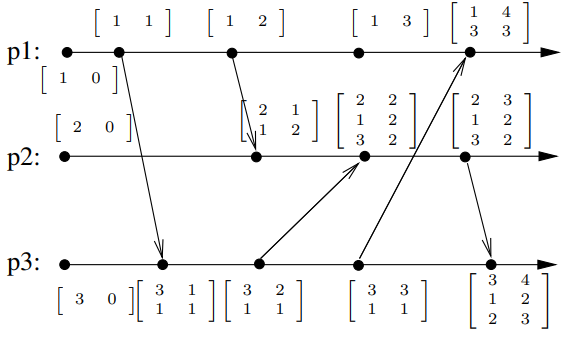
\includegraphics[width=\textwidth]{./rvd01.png}
            \caption{Reloj vectorial dinamico.}\label{fig:Deteccion.}
            \label{fig:Relojes vectoriales dinamicos}
        \end{subfigure}
    \end{figure}    
\end{frame}